\chapter{序論}
序論では,オーディオブックブックの市場や音声合成について解説し,朗読システムの課題を指摘し,本研究の目的や構成を述べる

\section{背景}
\subsection{オーディオブックの市場拡大と課題}
%社会的背景
近年,従来の紙の書籍以外にも電子書籍といった様々な書籍の楽しみ方が増えている.
その中でもオーディオブックは近急速な成長をしており,今後も成長が見込まれている.
オーディオブックとは書籍の朗読は専門のナレーターによる朗読音声を収録したものである.
もともと車社会のアメリカなどの国では早期から大きな市場を確立している.
近年インターネットを介したダウンロード販売が可能になったことなどによりさらに市場は拡大している.
アメリカとカナダの市場規模が2015年には前年比で約21\%拡大している\cite{wsj}.

日本においては,欧米に比べて小規模なものにとどまっている.
1980年代後半に後半にカセットブックが流行したが,車社会のアメリカに比べ電車などの公共機関による移動が多い日本では,市場規模はなかなか拡大しなかった.
しかし,近年,スマートフォンなどが普及しカセットを持ち歩かなくても気軽に楽しめる環境が整ったことにより,インターネット上のダウンロード販売が急速に拡大している.
日本の市場規模は2016年現在50億円程度と言われており,約10年後には800億円〜900億円ぐらいに見込まられるとされてる.\cite{cnet}

しかし,このようなオーディオブックは書籍から音声化する際には電子書籍化にくらべて非常に手間やコストがかかる.
声優の選定からはじまり録音や読み間違え確認,BGM挿入,再度録音など人での作業が多い.
そのため2〜3ヶ月ほどかかるを要し,コストは電子書籍の10倍ほどかかっていると言われている.\cite{ueda}

\begin{figure}[ht]
  \begin{center}
    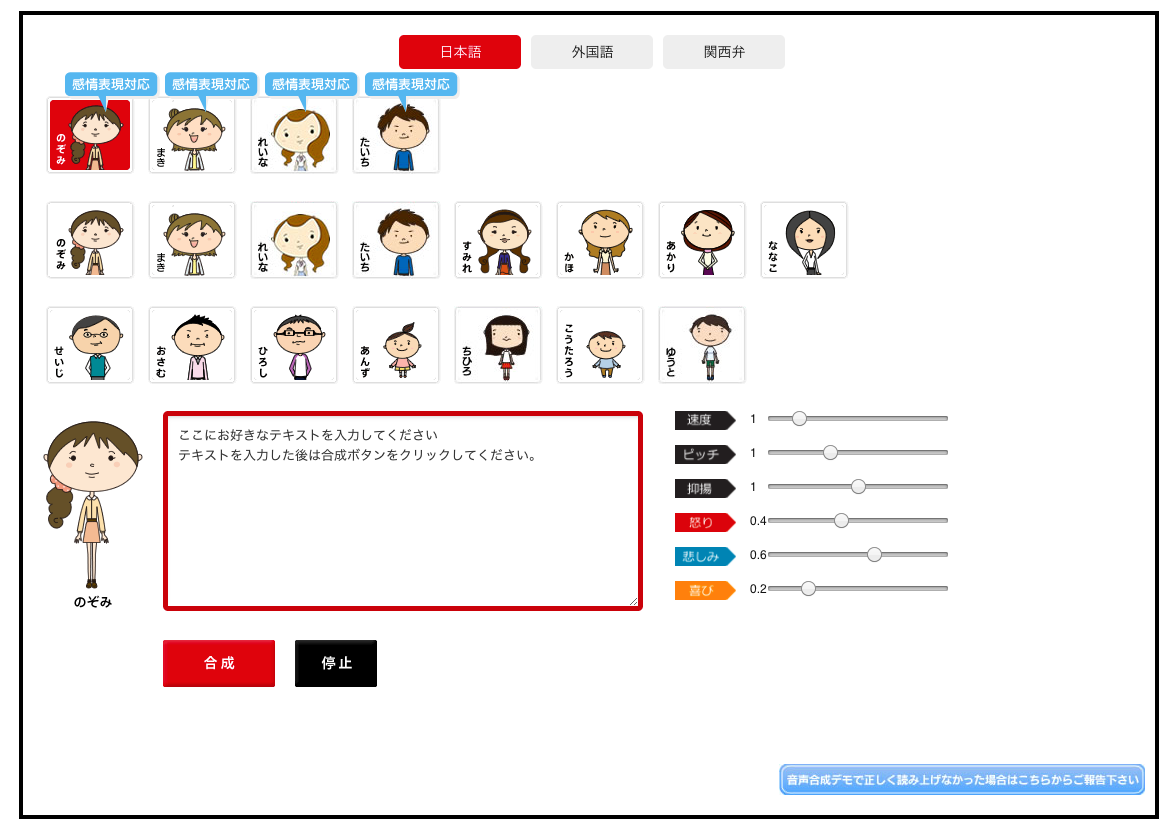
\includegraphics[clip,width=15.0cm]{fig/ai_talk.eps}
    \caption{感情表現可能な音声合成ソフトの例(AITalk)}
    \label{fig:ai_talk}
  \end{center}
\end{figure}

\subsection{音声合成技術の発展}\label{subsec:speech_synthesis}
音声合成とは,人間の音声を人工的に作り出すことである.
この技術は文字を読むことが困難な障害者,外国人や幼児などに画面読み上げソフトとして長く利用されてきており,言葉を発することが困難な人が代替手段として利用することも多い.
さらに,21世紀に入ってからは家電製品の音声ガイダンスや公共交通機関のアナウンス,ロボットの発話用途などとして広く使用されるようになっている.
近年では声の切り替えや声の高さの調整などが可能になり,さらには指定した感情で音声合成ができるシステムも実用化されている.
例えば,株式会社エーアイのAITalkは図\ref{fig:ai_talk}に示すように怒り・悲しみ・喜びの感情をそれぞれ10段階で指定して合成することが可能である.

\subsection{朗読システムの現状と課題}\label{subsec:reading_system}
音声合成技術を用いることで,物語の自動朗読システムを実現することは可能であり,実際に実用化されている.
しかし,品質は人間が読み上げて録音したものには及ばないのが現状である.
単に音声合成を使うだけではなく,物語にあわせて読み上げる朗読に特化したシステムが実用化されている例は筆者が知る限り存在しない.


このようなシステムの実現が難しい理由としていくつか考えられる.
まず,そもそもの音声合成の質の問題である.
音声合成を情報提供を目的としたアナウンスとして用いる場合は問題がなかったとしても,物語といった長文の場合には平坦で淡々とした読み上げになってしまう.
次に,朗読におけるポーズ長の重要性である.
章立てやパラグラフといった文章構造の他に意味内容によるポーズが重要であることが杉藤ら\cite{sugifuji}によって示されている.
意味内容まで考慮したポーズ長の推定は現状では難しいと考えられる.
最後に感情表現の問題である.
\ref{subsec:speech_synthesis}で述べたように,音声合成自体は感情表現が可能になった.
しかし,感情は人の手によって調整する必要があり,物語といった長文の場合はコストがかかる.
文章から自動的に感情を推定して,その推定された感情にしたがって読み上げる朗読システムは実用化されていない.
一方,テキストマイニングの分野で盛んに感情推定が行われているが,あくまで商品や映画などのレビューやクレームといった事実に対する感情を推定するものが多い.
そのため物語の文章に対してそのまま適応できるかは疑問である.
さらに,朗読の場合の感情推定は文中の人物の感情を推定するのではなく,あくまでどの感情表現で読むべきかを推定する必要がある.


\section{本研究の目的}
本研究では\ref{subsec:reading_system}で述べた朗読システムの課題の中で,感情推定の問題を取り扱う.
すなわち,朗読システムのために,未知の文に対しその文を読み上げるときの感情として最適なものを推定することを目的とする.
これにより音声合成システムの感情パラメータを自動的に調整することが可能になり,より自然な読み上げが自動的に行えるようになる.
さらに,自然な朗読システムが可能が実現可能になることで,人手での手間やコストをかけずにオーディオブックを作成できるようになることが期待される.


%%目的を達成するための手法
本研究では,文にどのような単語が含まれているかという出現情報をもとに機械学習技術を用いて感情を推定する.
名詞,動詞,形容,形容動詞は内容語とよばれるが物語に依存する可能性が高いため,内容を除いた機能語を用いることで内容に依存しない分類器を生成できる.
このため内容語を無視して機能語のみを用いて学習し感情の推定を行う.
セリフのみに限らずすべての文を対象に,出現情報から機能語に絞った感情推定を行っている研究は筆者の知る限り存在しない.


%%実験手法の正しさの確認
本研究では,先行研究に従いNormal,Happy,Sad,Angryの4つに感情をクラス分けする.
本手法の正しさを確認するための実験として,まず一つの文にそれぞれ4つの感情で音声を合成する.
そしてWebのアンケートシステムを用いて,被験者にこれらの音声を実際に聞いてもらい,その文を読み上げる際にどの感情が最も適しているか判定してもらう.
このように生成された学習データを用い交差検証を行うことで本手法の分類性能を評価する.


\section{本論の構成}
本章では,本論文の背景となるオーディオブック市場の拡大と音声合成技術を説明した上で朗読システムの現状と課題について説明し,それを踏まえ本研究の目的を述べた.
第2章では既存の関連する研究について述べる.
また第3章では本論文が提案する手法の詳細を述べ,第4章でその評価実験について説明する.
そのうえで第5章で提案手法の効果を測定するために行なった実験の結果と考察を述べ,第6章でその結論と今後の展望について述べる.

